\documentclass[12pt,twoside, a4paper, twocolumn]{article}
\usepackage[utf8]{inputenc}
\usepackage[brazil]{babel}
\usepackage[margin = 0.5in]{geometry}
\usepackage{amsmath}
\usepackage{amsthm}
\usepackage{amssymb}
\usepackage{amsthm}
\usepackage{setspace}
\usepackage[americanvoltages,fulldiodes,siunitx]{circuitikz}
\usepackage{lipsum}
\usepackage{pgfplots}
\usepackage{ifthen}
\usepackage{adjustbox}
\usepackage[section]{placeins}
\usepackage{hyperref}
\usepackage{graphicx}
\usepackage{adjustbox}
\pgfplotsset{compat=newest}
\graphicspath{ {./images/} }
%  #1 color - optional #2 x_0 #3 y_0 #4 x_f #5 y_f #6 name - optional  #7 true if adding lines to axis
\newcommand{\drawvector} [9] [color=cyan] {
\draw[line width=1.5pt,#1,-stealth](axis cs: #2, #3)--(axis cs: #4, #5) node[anchor=south west]{$#6$};
\ifthenelse{\equal{#7}{true}}{
\draw[line width=1pt,#1, dashed](axis cs: #4, #5)--(axis cs: #4, 0) node[anchor= north west]{$#8$};
\draw[line width=1pt,#1, dashed](axis cs: #4, #5)--(axis cs: 0, #5) node[anchor=south east]{$#9$};
}
{}
}
\newcommand\deriv[2]{\frac{\mathrm d #1}{\mathrm d #2}}
\title{Nono  Relatório de Física Experimental 2}
\author{Henrique da Silva \\ hpsilva@proton.me}
\date{\today}
\pgfplotsset{width = 10cm, compat = 1.9}
\begin{document}
\maketitle
\pagenumbering{gobble}
\newpage
%pagenumbering{roman}
\tableofcontents
\newpage

\section{Introdução}

\paragraph*{Neste relatório, vamos discutir propriedades de lentes, e lentes em série.}

\paragraph*{Também discutiremos alguns circuitos retificadores com diodos.}

\paragraph*{Todos arquivos utilizados para criar este relatório, é o relatório em si estão em:  \url{https://github.com/Shapis/ufpe_ee/tree/main/4th semester/}}


\section{Formação de imagens}

\paragraph*{Todos testes abaixo foram realizados com uma lente esférica de distância focal de 100mm.}

\subsection{Análise de distância com imagens nítidas}

\subsubsection{Teoria}

\begin{equation}
  \frac{1}{S} + \frac{1}{S'} = \frac{1}{f}
\end{equation}

\begin{equation}
  \begin{aligned}
     & D = S + S' = Sf - \frac{Sf}{S - f}                                            \\
     & \deriv{D}{S} = 1 + \frac{f(S-f) - Sf}{(S-f)^2} = \frac{-f^2}{(s-f)^2} + 1 = 0 \\
     & \frac{f^2}{(s-f)^2} = 1 \rightarrow \frac{f}{S-f} < 1 \rightarrow S = 2f      \\
     & D_{min} = 2f + \frac{(2f)^2}{f} = 4f
  \end{aligned}
\end{equation}


\subsubsection{Explicacao}

\subparagraph*{Podemos observar imagens nítidas com duas configurações diferentes de $S$ e $S'$.}

\subparagraph*{Este resultado vem diretamente das equações (1) e (2) acima.}

\subparagraph*{Como podemos observar. O $S$ e $S'$ são comutativos e a distância mínima para termos imagens é de $4f$. Ou seja. No nosso caso de $40cm$}

\subparagraph*{Com o espaço que temos para variar a posição do $S$ e do $S'$ na bancada, que é aproximadamente pouco mais de 40 centímetros. Nós teríamos no máximo duas imagens nítidas.}

\subparagraph*{Com a imagem nítida medimos $S = 15 \pm 1cm$ e $S' = 25 \pm 1cm$. e $S = 25 \pm 1cm$ e $S' = 15 \pm 1cm$}

\subparagraph*{Que era de fato o resultado esperado, já que isto nos dá um $S+S' = 40$. E satisfaz a equação (1).}

\subsubsection{Amplificacao}

\subparagraph*{Medimos amplificações diferentes nas duas configurações de imagem nítida.}

\subparagraph*{A imagem original tinha $0.7cm$. E medimos imagens formadas de $1cm$ e $0.3cm$}



\subsubsection*{Tabela de dados}

\begin{center}
  \begin{tabular}{ |c|c|c| }
    \hline
    $S \pm 1cm$ & $S' \pm 1cm$ & $S+S' \pm 2cm$ \\
    $15$        & $23$         & $38$           \\
    $17$        & $19$         & $36$           \\
    $19$        & $18$         & $37$           \\
    $21$        & $17$         & $38$           \\
    $23$        & $15$         & $38$           \\
    $25$        & $15$         & $40$           \\
    $27$        & $14$         & $41$           \\
    $29$        & $14$         & $43$           \\
    $31$        & $13$         & $44$           \\
    $33$        & $13$         & $46$           \\
    $35$        & $13$         & $48$           \\


    \hline
  \end{tabular}
\end{center}

\subsubsection*{Distancia focal da lente}


\begin{adjustbox}{scale=0.70}
  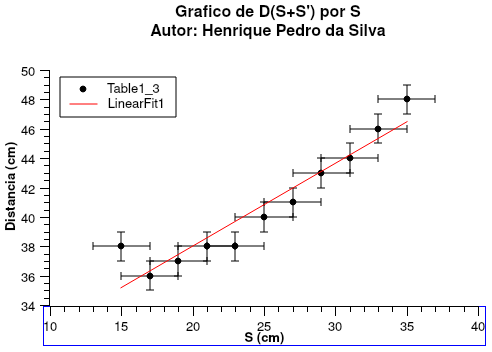
\includegraphics{Graph1.png}
\end{adjustbox}

\subparagraph*{Fazendo $\sum_{i=1}^{11} \frac{D_n}{n} = 4f$.}

\subparagraph*{Temos que $f_{experimental} = 10.2045$}

\subparagraph*{$\frac{\varDelta f}{f}$ nos dá um erro de  $2\%$}

\section{Telescopios}

\subsection{Diametro do laser}

\subparagraph*{Obtivemos um diâmetro de $0.70 \pm 0.05mm$ sem amplificação das lentes. E de $5.40 \pm 0.05mm$ com as lentes.}

\subparagraph*{Ou seja, uma amplificação de aproximadamente $8$ vezes.}

\subsection*{Projeção do laser na parede}

\subparagraph*{A divergência com as lentes foi significantemente menor do que sem as lentes.}

\subsection{Telescopios Kepleriano e Galileano}

\subparagraph*{Observamos em ambos telescópios uma amplificação da imagem.}

\subparagraph*{O telescópio Galileano tem a vantagem de ter dimensão transversal menor. Ou seja, as suas lentes estão mais próximas uma da outra devido a distância focal de uma das lentes ser negativa.}

\subparagraph*{O telescópio Kepleriano tem a vantagem da imagem que o observador tenta ver ser formada mais próxima da lente do que no Galileano. Ou seja. O espaço "atrás" do telescópio para o observador é menor.}

\subsection{Representacoes}

\begin{adjustbox}{scale=0.70}
  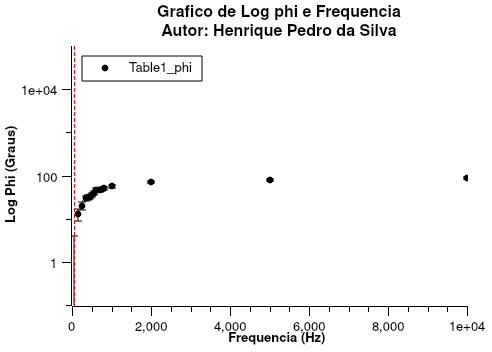
\includegraphics{Graph2.png}
\end{adjustbox}

\begin{adjustbox}{scale=0.70}
  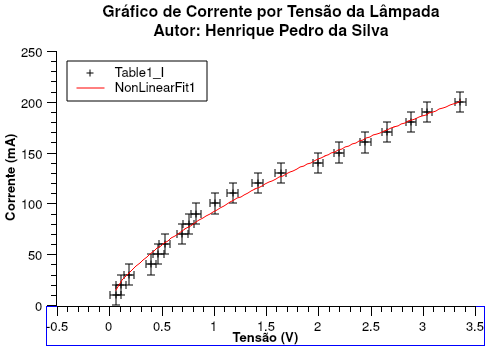
\includegraphics{Graph3.png}
\end{adjustbox}




\end{document}